\documentclass{article}

\usepackage{epsfig}
\usepackage{hyperref} 
\usepackage{graphicx}
\usepackage{listings}
\usepackage{color}

\definecolor{dkgreen}{rgb}{0,0.6,0}
\definecolor{gray}{rgb}{0.5,0.5,0.5}
\definecolor{mauve}{rgb}{0.58,0,0.82}

\lstset{frame=tb,
  language=C++,
  aboveskip=3mm,
  belowskip=3mm,
  showstringspaces=false,
  columns=flexible,
  basicstyle={\small\ttfamily},
  numbers=left,
  numberstyle=\tiny\color{gray},
  keywordstyle=\color{blue},
  commentstyle=\color{dkgreen},
  stringstyle=\color{mauve},
  breaklines=true,
  breakatwhitespace=true,
  tabsize=3
}


\title{Parallel Apriori Based Frequent Subgraph Mining}
\author{Matthew Whitesides\\
  \large CS6402 Advanced Data Mining}

\begin{document}
\maketitle

\section{Introduction}
Frequent Subgraph Mining is a particular task involved in Data Mining, the goal is to look for regularly occurring portions of a graph within the same graph or a larger set of graphs in a graph database. There are a few particularly intensive aspects of subgraph mining and in this paper, we'll look at the challenge of implementing these processes in a multi-threaded parallel process. The first focus is in candidate generation, which is the process of creating subgraphs that have the potential of becoming frequent subgraphs. The second is in subgraph isomorphism, which involves actually determining if a subgraph exists in a given graph. Given any non-trivial graph sizes, these processes can require exponentially large amounts of memory and processing resources. Here we will see if we can speed up these methods any back implementing these methods to run in parallel on a CPU, with the idea that given enough processors, threads and memory could scale the results to larger systems. 

In the following paper, we will be looking at the creation, implementation, and results of a parallel frequent subgraph mining algorithm. The algorithm is a modification of a fairly common Apriori-based approach to FSM, we'll test what aspects of the algorithm cause the slowest down and implement them in a way that can be run asynchronously. We find later in the results that the speed improvements scale quite well. 

\section{Setup}
The application code for the following paper can be found at:

\href{https://github.com/mattwhitesides/CS6402-Final-Project}{https://github.com/mattwhitesides/CS6402-Final-Project}. 

The implementation was written in C++, with minimal external dependencies. The included external headers are, \href{https://math.nist.gov/~RPozo/graph/ngraph_index.html}{NGraph++} and \href{https://github.com/catching/Catch2}{Catch2}. NGraph++ is a simple header file that contains a lightweight Graph data structure with basic insert edge and gets vertex neighbor functionality. No mining algorithms or complex features are part of the NGraph code leaving a clean foundation as to not have too many issues from the implementation of a Graph data structure rather focusing on the mining algorithms. Catch2 is another header only lightweight unit testing framework that I used to help test and debug some of the code.

To compile the project you will need a C++ compiler gcc-g++ version 7.0 or later supporting C++17 features, and Make version 4.0 or later to build the makefile. To build and run the application on a Linux system simply clone the Git repo and run make, this will compline the multi-process application and can be run from the command line, with the following syntax: 
"./multi \{Dataset Directory Path\} \{Optional Min Support Threshold\} \{Optional Thread Count\}\{Optional Output File Name\}".
In addition you can run the command "make single" to make the non-threaded single process that contains no multi-threaded which essentially is similar to running the multi-threaded application with the thread count set to 1 however even that will still spawn a single new thread in the operating system and will wait for it finish so this version would have none of that overhead for a perfect comparison. Finally, you can run  "make test" to create the testing project to verify the application built correctly however this is unmessy for use. 

The first argument the dataset directory path expects a path to a folder containing a database of graph files. A graph file should contain a list of edges as numeric identifiers with a space separating them, for ex. "1 3" would be a line in the file indicating there is an edge between vertices 1 and 2. All files in the given directory will be read into the application as graph objects.

The second argument is a numeric for the minimum support threshold or simply how many occurrences of a given subgraph need to happen before it is considered a "frequent subgraph". 

The third is numeric for how many threads you want to spawn while running the application, the higher the number the more data will be processed in parallel for a standard modern CPU with 4 real cores and 8 hyperthreaded cores any value over 4 or so will see CPU usage near 100\%.

The fourth argument is the file path where you would like to print the detailed results of the mining.

Arguments two through four are optional and if you only include the first values of 2 in support, 2 threads, and subgraphs.txt will be given. 

\section{Implementation}

The basic Apriori-based method I wrote the method off of consists of first finding all frequent single subgraphs which are straightforward enough just look at every node and see if it occurs enough times. Then building upon there, in a loop while we are still finding frequent subgraphs will build a list of candidates off of the previous iteration then check if each candidate is contained in the database. Simply enough that's the basics of it and my implementation is as follows in figure 1 below. 

\begin{figure}
\begin{lstlisting}
/**
	Apriori-based approach for finding frequent subgraphs.

	@param g: the graph to be mined.
	@param s: the minimum support threshold.
	@return a vector list of the frequent subgraphs of cardinality 1 to k.
*/
vector<Graph> AprioriBased(vector<Graph> ds, int s) {
	int k = 2;
	vector<Graph> subGraphs;
	vector<vector<Graph>> f;

	f.emplace_back(vector<Graph>());		
	f.emplace_back(FrequentOneSubgraphs(ds, s));

	while (f[k - 1].size() != 0) {
		f.emplace_back(vector<Graph>());
		vector<Graph> c = CandidateGen(f[k - 1]);
		
		for (auto& g : c) {
			for (auto& gi : ds) {
				if (SubGraphIsomorphism(g, gi)) {
					++g.count;
					continue;
				}
			}

			if (g.count >= s && !GraphInSubGraphSet(subGraphs, g)) {
				subGraphs.emplace_back(g);
				f[k].emplace_back(g);
			}
		}
		k++;
	}

	return subGraphs;
}
\end{lstlisting}
  \caption{Single Threaded Aprori Based Approach.}
  \label{fig:Single Threaded Aprori Based Approach}
\end{figure}

To begin looking into parallel/multi-threaded processing we can start with one of the more intensive looping processes, candidate generation. Currently, the way our candidate generation looks is it iterates over each graph in the dataset starting with single frequent nodes, then iterates over it again joining each node to each other graphs nodes. This essentially is a (Number of Graphs\textsuperscript{2} + Number of Nodes\textsuperscript{2}) type of overhead (Figure 3).

Now we can think logically none of this modifies any data only adds to a list of candidates so we should be able to split this task up among multiple threads. First I'll attempt to make each graphs iteration its own thread, that'll mean lines 2 through 6 will operate independently. However even on a small dataset such as our randomly generated on we have at the start about 96 single vertex frequent subgraphs so in the smallest case that'll spawn 96 threads. It appears doing this along with the overhead of creating the threads, copying the data in memory again, and waiting for the threads to rejoin we have actually increased our runtime from, 8 seconds and 278 milliseconds in single threaded mode to 14 seconds and 766 milliseconds in multi-threads.

Maybe we simply have too many threads getting spawned, next let's see if we might be able to limit the number of threads that we're creating so we are still looping over multiple candidates however we'll split each process up into (\# Candidates)/(N \#Threads) candidates. This essentially puts the entire function Lines 1 through 7 into our desired N number of threads. This will require splitting out candidate list into N number of lists and spawning a thread for each subset. This implementation while it seems to get rid of the decrease in performance, it does not give us any improvement, we now have a runtime of 8 seconds and 579 milliseconds which is still worse on average. See Figure 3 for the implementation of multi-threaded candidate generation.

Next and what I should have done first is measure exactly where the longest running sections of the code are. Splitting up the Canidiate generation and the checking if the subgraph exists gives us these times. For a fuller breakdown of the long-running processes refer to figure 4 where we break down the percentage of the time required for each section, and note that "Check Candidates for Frequency" as the dataset grows takes up more and more of the time, it's only even in these smaller running times that you'll even notice the other aspects. (Figure 2)

We can see that roughly 6 out of the 8 seconds is just the checking to see if a candidate is a valid subgraph which requires essentially at worst scanning the entire graph to see if they match. However, we may be able to split this part up as we can check multiple graphs at a time. Also, note I'll be reverting the candidate generation back to single threaded just for continuity sake. Unfortunately, upon the first attempt, I'm getting worse times around 
3 minutes, and only found 73 subgraphs, which is about 18 times slower and half as accurate. Some more work will need to be done, perhaps we're running into a false memory thread constraint. Turns out the issue with finding fewer subgraphs was due to a logic error in the splitting of the data into multiple sets, however once fixing that we still have the issue of it taking, well actually now about 30x longer as it's finding all the subgraphs. Upon trying a variety of measures to assure that no memory is shared between threads it appears there are known issues with Cygwin on multi-core Windows machines not being able to utilize multiple threads. When I attempt to run the application through Windows and build with the Visual C++ compiler we do see an increase in performance when adding multiple threads which we'll look at in the performance section.

So the final idea behind the multi-threaded implementation is instead of looking at each of the candidates in a sequence we can look at multiple candidates at a time, we often have hundreds and thousands of candidates especially in the early levels one and two before the candidates can start getting weeded out. Here on line 25 (Figure 5) well split up the candidate dataset into equal parts for the given number of threads we want to create and each thread will check to see that the candidates exist in the graphs and once each thread is done they will join results at the end before moving to the next k-level of the loop.

\begin{figure}
  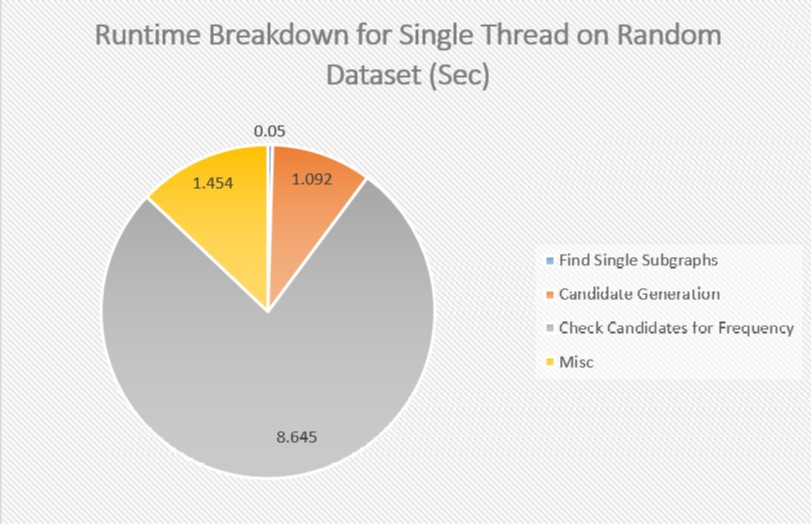
\includegraphics[width=\linewidth]{Figure2.jpg}
  \caption{Runtime Breakdown.}
  \label{fig:Runtime Breakdown}
\end{figure}

\begin{figure}
\begin{lstlisting}
/**
	Generates a list of candidates for a frequent subgraph using a modified level-wise join.

	@param g: The graphs being considered.	
*/
vector<Graph> CandidateGen(vector<Graph> ds) {
	vector<Graph> candidates;

	for (Graph& g : ds) {
		candidates.emplace_back(g);
		for (Graph::const_iterator p = g.begin(); p != g.end(); p++) {
			for (Graph& g2 : ds) {
				for (Graph::const_iterator p2 = g2.begin(); p2 != g2.end(); p2++) {
					auto node1 = Graph::node(p);
					auto node2 = Graph::node(p2);
					if (node1 != node2) {
						auto c = g;
						c.insert_undirected_edge(node1, node2);
						candidates.emplace_back(c);
					}
				}
			}
		}
	}

	return candidates;
}
\end{lstlisting}
  \caption{Single Threaded Candidate Generation.}
  \label{fig:Single Threaded Candidate Generation}
\end{figure}

\begin{figure}
\begin{lstlisting}
/**
	Generates a list of candidates for a frequent subgraph using a modified level-wise join.

	@param g: The graph being considered.
	@param s: The minimum support threshold.
	@param f: The single subgraph to start off of.
	@return: A vector list of the frequent subgraphs.
*/
vector<Graph> CandidateGen(vector<Graph> ds, int t = 1) {
	vector<Graph> candidates;
	auto subVectors = SplitVectorIntoSubVectors(ds, t);

	for (Graph& g : ds) {
		vector<thread> threads;
		vector<future<vector<Graph>>> futures;
		candidates.emplace_back(g);

		for (auto& sg : subVectors) {
			promise<vector<Graph>> p;
			futures.emplace_back(p.get_future());
			threads.emplace_back(thread(AddCandidates, g, sg, move(p)));
		}

		for (auto& t : threads) {
			t.join();
		}

		for (auto& f : futures) {
			for (auto& g : f.get()) {
				candidates.emplace_back(g);
			}
		}
	}

	return candidates;
}
\end{lstlisting}
  \caption{Multi Threaded Candidate Generation.}
  \label{fig:Multi Threaded Candidate Generation}
\end{figure}

\begin{figure}
\begin{lstlisting}
/**
	Apriori-based approach for finding frequent subgraphs.

	@param g: The graph to be mined.
	@param s: The minimum support threshold.
	@param t: The minimum support threshold.
	@return: A vector list of the frequent subgraphs of cardinality 1 to k.
*/
vector<Graph> AprioriBased(vector<Graph> ds, int s, int t = 1) {
	unsigned int k = 2;
	vector<Graph> subGraphs;
	vector<vector<Graph>> f;

	f.emplace_back(vector<Graph>());
	f.emplace_back(FrequentOneSubgraphs(ds, s));

	while (f[k - 1].size() != 0) {
		f.emplace_back(vector<Graph>());

		vector<Graph> c = CandidateGen(f[k - 1], t);

		vector<thread> threads;
		vector<future<vector<Graph>>> futures;
		auto subCandidates = SplitVectorIntoSubVectors(c, t);

		int ti = 1;
		for (auto& sc : subCandidates) {
			promise<vector<Graph>> p;
			futures.emplace_back(p.get_future());
			threads.emplace_back(thread(AddCandidateIfValid, sc, ds, s, ti, move(p)));
			++ti;
		}

		for (auto& t : threads) {
			t.join();
		}

		for (auto& future : futures) {
			for (auto& g : future.get()) {
				if (!GraphInSubGraphSet(subGraphs, g)) {
					subGraphs.emplace_back(g);
					f[k].emplace_back(g);
				}
			}
		}
		
		k++;
	}

	cout << endl;
	return subGraphs;
}
\end{lstlisting}
  \caption{Multi Threaded Aprori Approach.}
  \label{fig:Multi Threaded Aprori Approach}
\end{figure}

\pagebreak

\section{Results}

The dataset used in testing include the \href{http://snap.stanford.edu/data/ego-Twitter.html}{Social circles: Twitter} a dataset of Twitter users friends connections, \href{http://snap.stanford.edu/data/ego-Facebook.html}{Social circles: Facebook} a dataset of Facebook survey participants, and a Randomly generated dataset that consists of IDs 0 - 100. One note is the Twitter dataset contains 973 graphs however only the first 35 were used for sake of time, as well as the minimum support threshold,  was increased to 3 for the larger datasets. Refer to figure 6 for details on the datasets.

The hardware used was run on a machine with an Intel i7-4810MQ @ 2.8GHz processor with 4 Cores and 8 Logical cores, and contains 16 GB of RAM.

The results are actually quite good for each thread we see roughly a 50\% performance increase however the increase declines exponentially as the threads increase. Likely due to the hardware being used that it cannot on a hardware level utilize more than 8 processes at a time and surely the operating systems doing background stuff at the same time we see pretty consistently there is almost performance gain above 5 threads. Also, note that while processing the CPU usage on the machine is maxed out, however, we might be able to hypothesize from this that given more cores to be used we would be able to continue to increase our performance in a similar way to threads 1-4.

\begin{figure}
  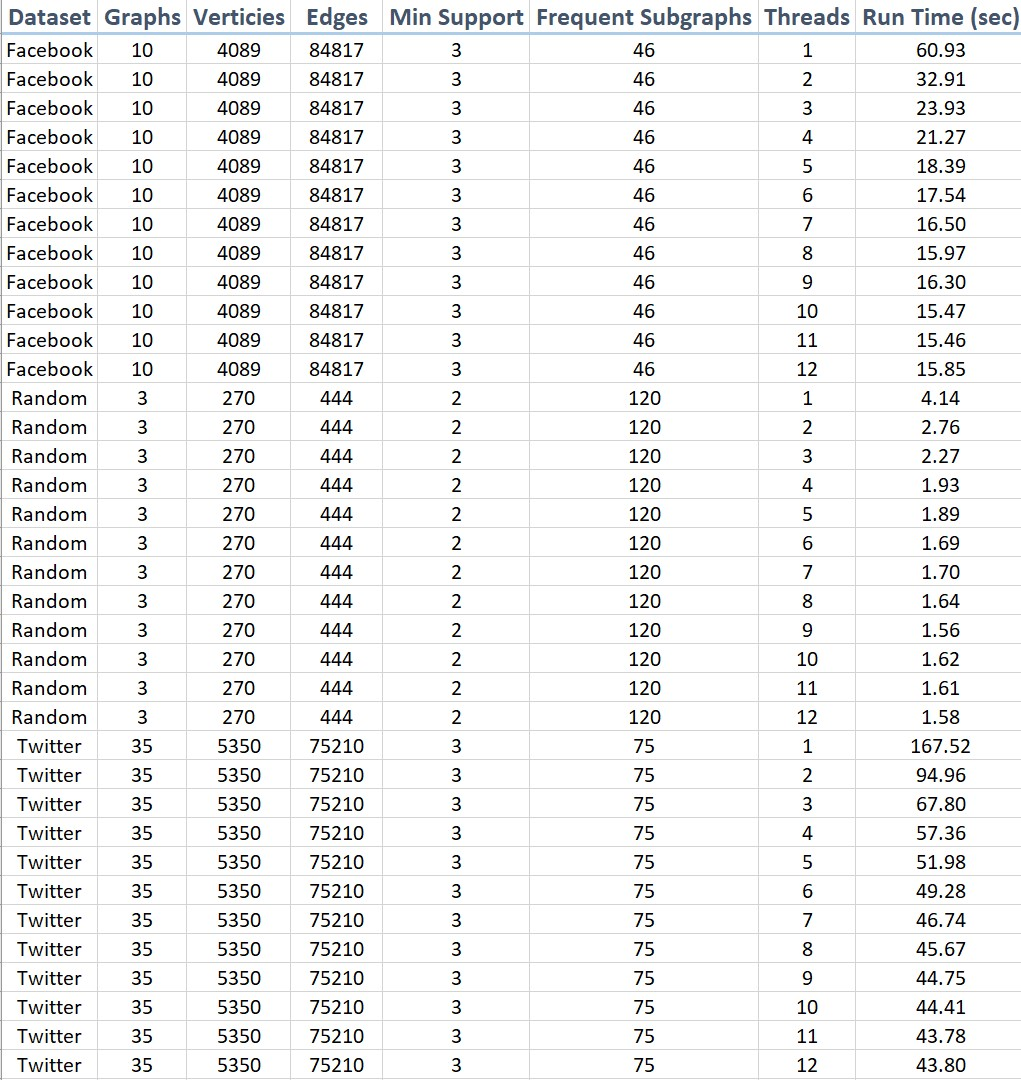
\includegraphics[width=\linewidth]{Figure6.jpg}
  \caption{Testing Results.}
  \label{fig:Testing}
\end{figure}

\begin{figure}
  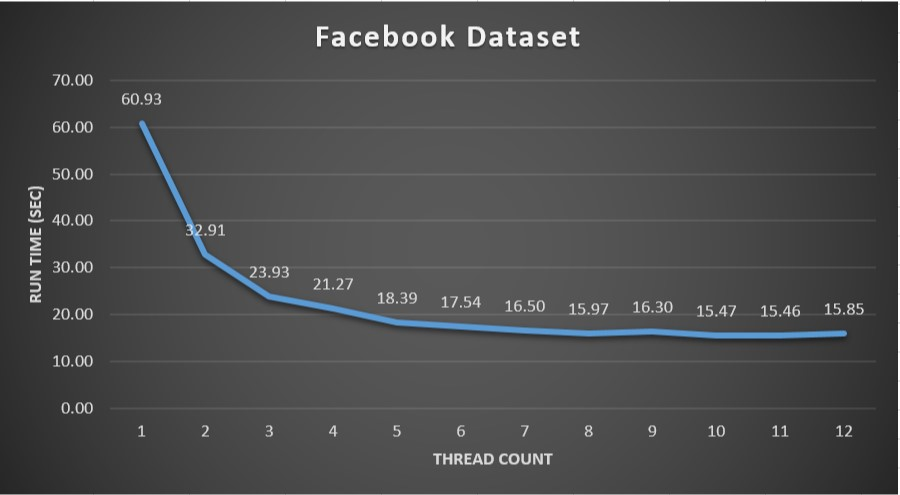
\includegraphics[width=\linewidth]{Figure7.jpg}
  \caption{Facebook Dataset Results.}
  \label{fig:Facebook}
\end{figure}

\begin{figure}
  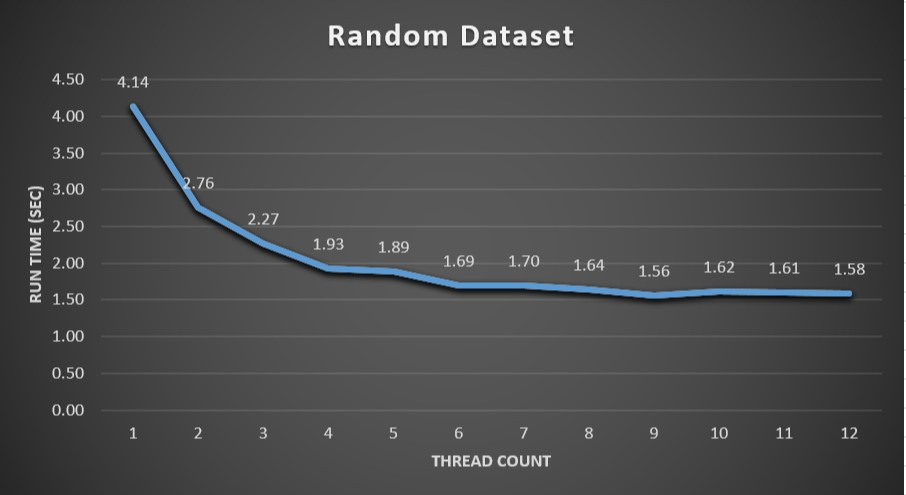
\includegraphics[width=\linewidth]{Figure8.jpg}
  \caption{Random Dataset Results.}
  \label{fig:Random}
\end{figure}

\begin{figure}
  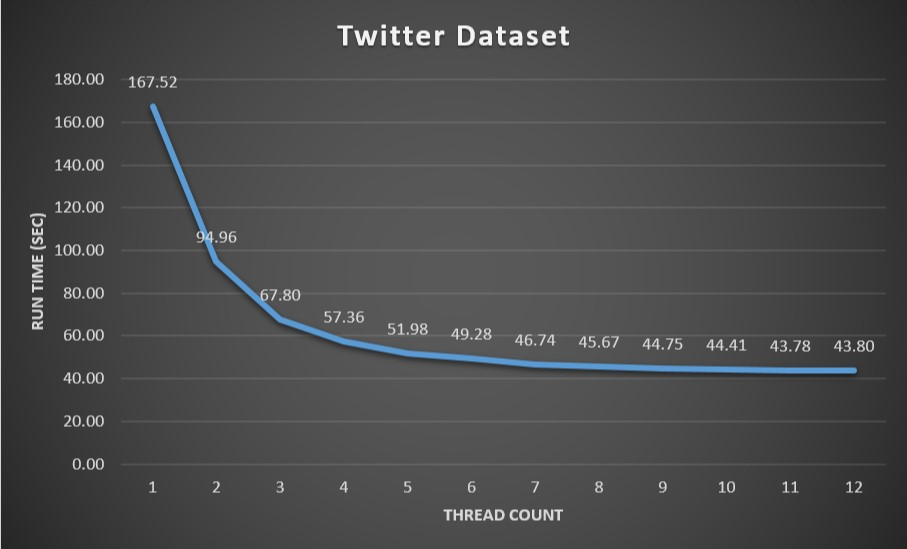
\includegraphics[width=\linewidth]{Figure9.jpg}
  \caption{Twitter Dataset Results.}
  \label{fig:Twitter}
\end{figure}

\end{document}